\chapter{Methodik}
\label{ch:methodik}

\section{Extraktion von Diagrammen aus Texten}

Ziel des ersten Teils ist die Extraktion der Diagrammen aus den historischen Textscans, welche dann im folgenden Teil in eine gewünschte Form ausgewertet werden können.
\\
Die Wesentlichen Schritte des Extraktionsteils beinhalten die Objekterkennung, also die Bestimmung des Begrenzungsrechtecks (bounding box) der Diagrammen innerhalb den vorliegenden Vollseitscans und deren Unterscheidung in verschiedene Diagrammtypen, beispielsweise Linien- und Balkendiagrammen.
Die erkannten Liniendiagramme werden anschließend anhand ihrer Auswertungsschwierigkeit klassifiziert, etwa durch Kennzeichnung deren Diagrammen, welche kontextbedingt gruppiert wurden, zum Beispiel aufgrund gemeinsamer Graphsachsen.

% \subsection{Erkennung von Diagrammen in Texten}
Um mit Hilfe von Deep-Learning Modelle zu trainieren, werden annotierte Grundwahrheiten (ground truth) benötigt.

\subsection{Datensatz DocBank zur Objekterkennung}
\label{ch:chartbank}

Für die Erkennung von Diagrammen in Texten wurden DocBank \cite{li2020docbank} und ein Anteil der historischen Wirtschaftsscans verwendet. DocBank besteht aus wissenschaftliche Publikation mit computergenerierten Grafiken zusammengesetzt, weshalb DocBanks Dokumentenseiten lediglich zum Vortrainieren des Detektionsmodells gedacht sind. Beabsichtigt wurde dieser Prozess des Vortrainierens um das System schneller und algemeingültiger, also mit besseren Voraussagen, trainieren zu können. Spätere Experimente untersuchen diese Annahme.
\\
An die Vorkommenshäufigkeit bei den historischen Scans angepasst, wurde die Differenzierung in fünf Objektklassen beschlossen: Linien (line), Balken (bar), Histogramm (histogram), Sonstige (other) und Gemischt (mixture). Aufgrund von Verwechslungen des Modells im Verlauf der Experimente zwischen Balkendiagrammen und Histogrammen wurden die Datensätze auf vier Klassen reduziert, indem Balkendiagramme und Histogramme vereinigt wurden.
\\
Die Schwierigkeit zwischen Balkendiagrammen und Histogrammen zu unterscheiden beruht darauf, dass Balkendiagramme kategorische Datenvergleiche anschaulich machen, bei denen die Balkenanordnung irrelevant ist, während Histogramme kontinuierliche, numerische Daten darstellen. Die Differenz liegt lediglich an der Achsenbeschreibung und nicht an visuellen Hinweisen, oftmals werden Balkendiagramme jedoch mit Lücken zwischen den Balken dargestellt, während Histogramme lückenlos abgebildet werden; dies ist allerdings nicht ausschlaggebend zur Bestimmung des Diagrammtyps.
\\
Für die manuell GT-Annotation der DocBank Dokumentenseiten, sowie folgender anderer Datensätze, wurde die Annotationssoftware CVAT \cite{CVAT_ai_Corporation_Computer_Vision_Annotation_2023} verwendet.

\begin{figure}[H]
    \centering
    \captionsetup{width=.75\linewidth}
    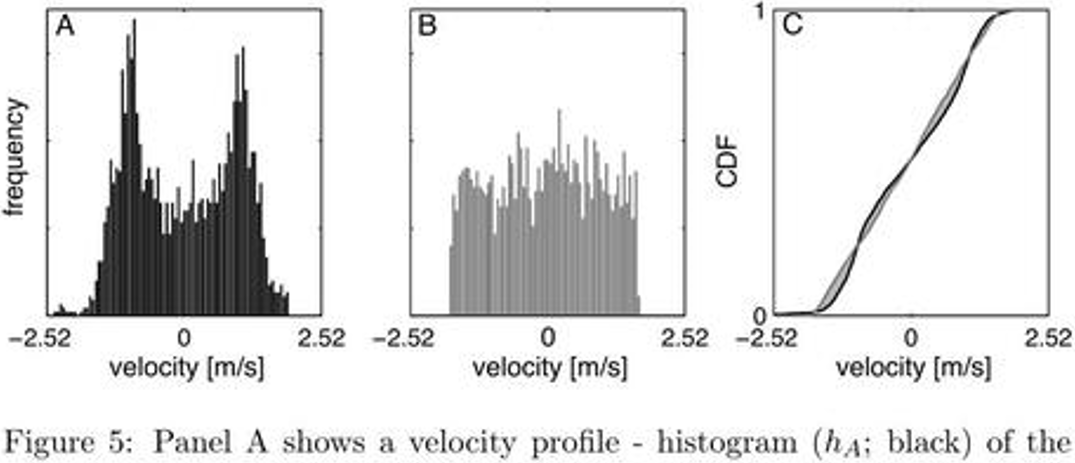
\includegraphics[width=.75\textwidth]{Methodik/img/docbank_example.png}
    \caption{\hbadness=10000 Beispiel kontextbedingter Gruppierung wegen gemeinsamer Y-Achsenbeschreibung eines gemischten Diagrammtyps (Histogramm und Liniendiagramm)}
    \label{fig:docbank_example}
\end{figure}

Da der Datensatz aus einer beträchtlich diversen Menge verschiedener wissenschaftlichen Publikationen besteht, beinhalten diese auch zahlreich verschiedene Diagrammlayouts. Um eine bestmögliche Konsitenz und Nützlichkeit in der Handannotation zu gewährleisten wurden einige Überlegungen gemacht: Da einige Abbildungen als Gruppe von Diagrammen fungieren, siehe Abbildung \ref{fig:docbank_example}, muss die generelle Entscheidung getroffen werden, jedes Diagramm der Gruppe einzeln zu annotieren oder lediglich die gesamte Gruppe zusammen. Beide Möglichkeiten liefern Vor- und Nachteile; beim getrennten Annotieren muss die Gruppe in einem späteren Schritt nicht mehr in die einzelnen Diagramme aufgeteilt werden, jedoch können auch kontextbedingte Informationen verloren gehen, wie in dem abgebildeten Beispiel die Y-Achsenbeschreibung des mittleren Diagramms (B), welches sich eine gemeinsame Y-Achsenbeschriftung mit dem linken Diagram (A) teilt.
Ebenfalls können Diagrammgruppen aus verschiedenen Diagrammtypen bestehen, etwa Histogramme und Liniendiagramme beieinander, weswegen dementsprechend für genau diesen Fall die gemischte Diagrammklasse eingeführt wurde. Bei weiteren Unklarheiten des Gruppenumfangs wurde sich sonst immer an die darunterliegenden Abbildungsunterschrift gehalten.
\\
Insgesamt wurden 321 Seiten annotiert, beinhaltend aus 105 Liniendiagrammen, 115 Balkendiagrammen (vereinigt mit Histogrammen), 79 sonstige und 66 gemischte Diagrammen.

\subsection{Datensatz historischer Wirtschaftsscans zur Objekterkennung}
\label{ch:scanbank}

\begin{wrapfigure}{r}{0.25\textwidth}
    \vspace{-\intextsep} % Remove vertical space above the figure
    \centering
    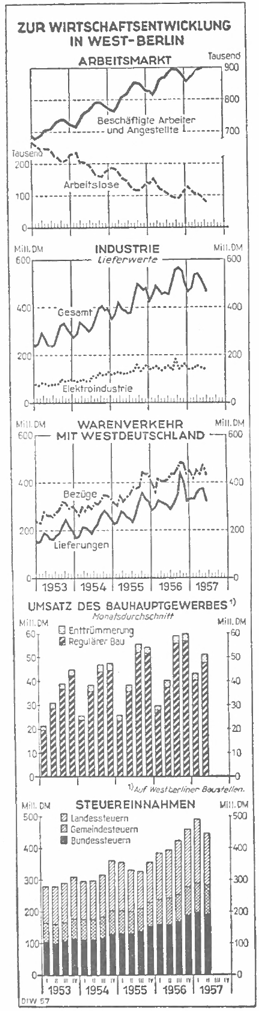
\includegraphics[width=\linewidth]{Methodik/img/scanbank_example.png}
    \caption{\hbadness=10000 Diagrammbeispiel historischer Scans}
    \label{fig:scanbank_example}
\end{wrapfigure}

Die Scans der geschichtlichen Wirtschaftsmagazine wurden mit ähnlichen Überlegungen annotiert. Hier befinden sich ebenfalls Diagrammgruppen, teils auch mit mehreren verschiedenen Diagrammtypen, siehe Abbildung \ref{fig:scanbank_example}, welche alle wieder als gesamte Gruppe annotiert wurden. Bis auf sehr wenigen Ausnahmen, befinden sich alle Abbildungen in den Scans visuell eingerahmt. Da die Ausrichtung derer jedoch nie wirklich perfekt gerade dargestellt wurde, und somit, der Ausrichtung verschuldet, kein Annotationsrechteck mit ausgeschlossenem Abbildungsrahmen gezeichnet werden kann wurde die Entscheidung getroffen, jede Annotation mit allen Ecken der Diagrammrahmen zu beinhalten. Grunsätzlich wurden alle Abbildungen, Diagramme oder nicht, wie etwa vereinzelte Karikaturen oder Landedskarten mit in die Klasse der sonstigen Diagramme eingeschlossen um so die allgemeine Erkennung von seltenen Diagrammtypen zu verstärken.
Es wurden insgesamt 2391 zufällige Seiten ausgewählt und manuell annotiert, woraus sich 343 Liniendiagramme, 102 Balkendiagramme, 77 sonstige und 52 gemischte Diagramme ergebten.

\clearpage
\section{Schwierigkeitsklassifizierung von Liniendiagrammen}
\label{ch:linebank}

Aufgrund der überwiegenden Liniendiagrammen in den historischer Wirtschaftsscans, wurde sich im Folgenden primär auf die Auswertung der Liniendiagrammen fokusiert.
\\
Für genau diese Auswertung wurde der Vorverarbeitungsschritt überlegt, die extrahierten Liniendiagramme in verschiedene Untergruppen zu unterteilen. Es wurden vier Klassifikationen gewählt; Liniendiagramme mit nur einer Wertelinie, aus zusammengesetzten Diagrammen, also Liniendiagrammsgruppen, sich nicht überlappenden Wertelinien und sich überlappenden Wertelinien.

\begin{figure}[H] % or any other figure positioning (H, h, t, b)
    \centering
    \begin{minipage}{0.475\textwidth} % First figure
        \centering
        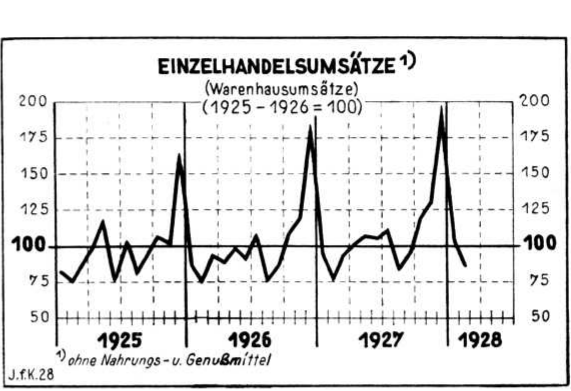
\includegraphics[width=\linewidth]{Methodik/img/linebank_single.png}
        \caption{\hbadness=10000 Liniendiagramm mit einer Wertelinie}
        \label{fig:linebank_single}
    \end{minipage}\hfill % Add space between figures
    \begin{minipage}{0.475\textwidth} % Second figure
        \centering
        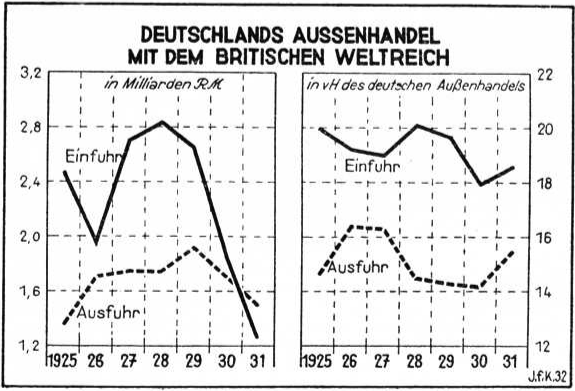
\includegraphics[width=\linewidth]{Methodik/img/linebank_composite.png}
        \caption{\hbadness=10000 Zusammengesetzte Liniendiagrammsgruppe}
        \label{fig:linebank_composite}
    \end{minipage}

    \vspace{0.75em}

    \begin{minipage}{0.475\textwidth} % First figure
        \centering
        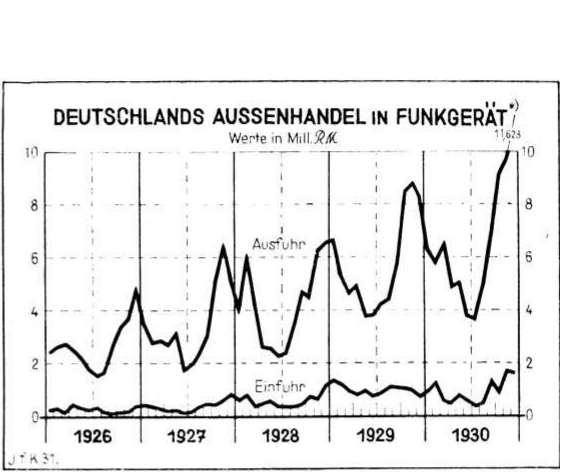
\includegraphics[width=\linewidth]{Methodik/img/linebank_non_overlapping.png}
        \caption{\hbadness=10000 Liniendiagramm mit sich nicht überlappenden Wertelinie}
        \label{fig:linebank_non_overlapping}
    \end{minipage}\hfill % Add space between figures
    \begin{minipage}{0.475\textwidth} % Second figure
        \centering
        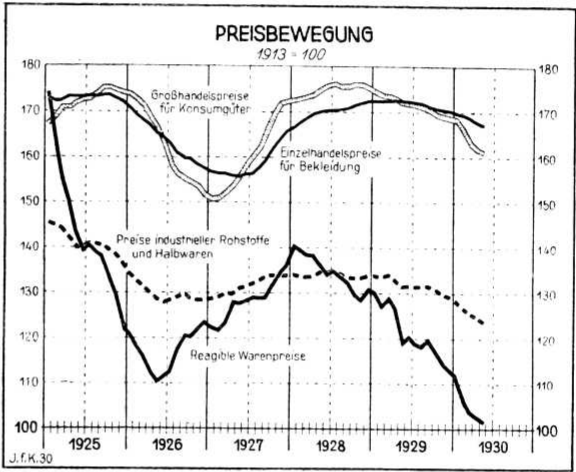
\includegraphics[width=\linewidth]{Methodik/img/linebank_overlapping.png}
        \caption{\hbadness=10000 Liniendiagramm mit sich überlappenden Wertelinie}
        \label{fig:linebank_overlapping}
    \end{minipage}
\end{figure}
Es existieren nämlich Liniendiagrammsgruppen mit mehreren eigenständigen Unterdiagrammen, welche möglicherweise jeweils ihre eigene Achsenbeschreibung haben, oder auch sich kontextbedingt diese Achsenbeschriftungen teilen. Diese müssen also im Vergleich zu einfachen Liniendiagrammen speziell behandelt werden. Aber auch wenn für Liniendiagramme mit nur einer oder sich nicht überschneidenden Wertelinien ein eher primitiver Extraktionsalgorithmus ausreichen würde, tritt bei komplexeren, sich überlappenden oder überschneidenden Wertelinien schnell das Problem der Linientrennung bzw. Liniengruppierung auf.
\\
Der erstellte Datensatz für die Schwierigkeitsklassifizierung besteht aus 807 klassifizierten Liniendiagrammen, unterteilt auf 93 mit einer Wertelinie, 284 zusammengesetzte, 94 nicht überlappendene und 336 überlappende Liniendiagramme.
\\
Eine zweite Version des Datensatzes wurde ebenfalls erstellt. Bei diesem wurde aufgrund späteren Klassifizierungsproblemen von sich nicht überlappenden mit überlappenden Wertelinien, beide Klassen in die gemeinsame Differenzierung der Liniendiagrammen mit mehreren Wertelinien vereinigt. Dementsprechend besteht die zweite Version des Datensatzes aus 430 Instanzen dieser Klasse.

\section{Auswertung von Liniendiagrammen}

Für die Auswertung der historischen Liniendiagramme wurden Überlegungen gemacht, Beschriftungen und vorallem das Hintergrundgitter, welches sich in jedem Diagramm zu finden lässt, zu entfernen, jedoch wurde schnell klar, dass diese primitive Herangehensweise grundsätzlich eher impraktibel ist. Zum einen führen die nicht genau senkrecht und waagerecht verlaufenden Gitterlinien die korrekte Erkennung dieser zu einem nichttrivialem Erkennungsproblem und zum andern überlappen und verlaufen viele Wertelinien auf dem Gitter, sodass die einfache Entfernung der Gitterlinienpixel das Diagramm mit unzähligen Lücken verbleiben lässt. Dementsprechend wurde beschlossen, statt aus dem Diagramm alles bis auf die Wertelinien zu entfernen, die Wertelinien selbst zu extrahieren, also sie durch Segmentation vom Hintergrundgitter und allen anderen Elementen zu trennen.
\\
Die manuelle Erstellung der Grundwahrheiten für die Werteliniensegmentation ist allerdings recht arbeitsaufwendig, weswegen zusätzlich ein synthetisch erstellter Datensatz generiert wurde, bei dem die Erstellung von Binärmasken der Wertelinien trivial ausfällt.
\\
Im Folgenden wird die Datensatzerstellung für die sowohl semantischer Segmentation, als auch Instanzsegmentation beschrieben. Die semantische Segementation benötigt pro Klasse nur eine gemeinsame Binärmaske, unabhängigt von der Anzahl der Objekte, also in dem Fall der Werteliniensegmentation eine Maske pro Liniendiagramm. In dem Fall der Instanzsegmentation dagegen, wird nicht nur eine eigene Maske pro jeweiliges Objektaufkommen - pro Objektinstanz - erfordert.

\clearpage

\subsection{Datensatz von synthetischen Liniendiagrammen zur Segmentation}
\label{ch:genlines}

\begin{figure}[H] % or any other figure positioning (H, h, t, b)
    \centering
    \begin{minipage}{0.475\textwidth} % First figure
        \centering
        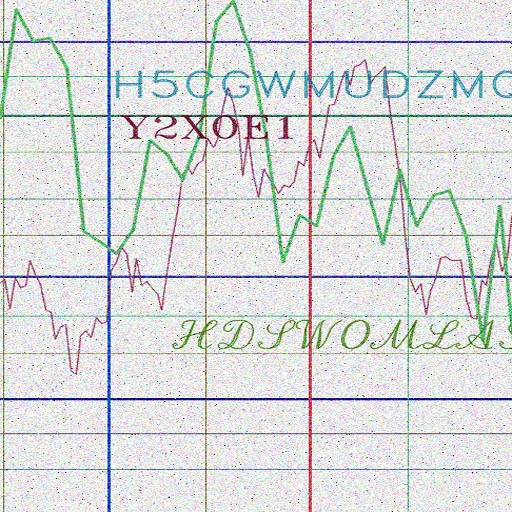
\includegraphics[width=\linewidth]{Methodik/img/lines_synthetic.png}
        \caption{\hbadness=10000 Synthetisch erstelltes Liniendiagramm}
        \label{fig:lines_synthetic}
    \end{minipage}\hfill % Add space between figures
    \begin{minipage}{0.475\textwidth} % Second figure
        \centering
        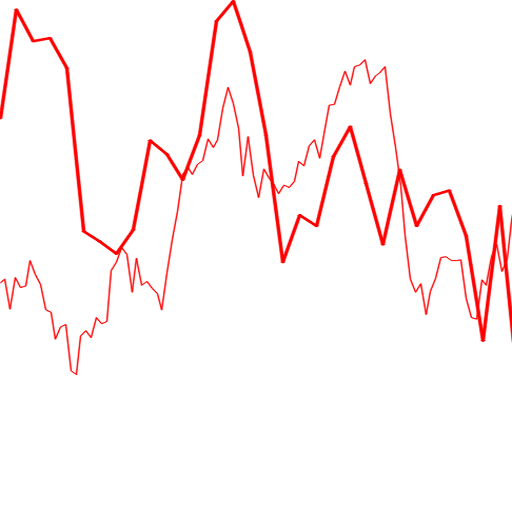
\includegraphics[width=\linewidth]{Methodik/img/lines_synthetic_mask.png}
        \caption{\hbadness=10000 Zugehörige generierte Binärmaske der Wertelinien}
        \label{fig:lines_synthetic_mask}
    \end{minipage}
\end{figure}

Der synthetische Datensatz besteht aus 2000 verschiedenen, zufällig generierten Liniendiagrammen. Diese beinhalten zufällige Wertelinien und Gitterlinien, sowohl in Position als auch in Liniendicke und beliebige, teils den Wertelinien überlappenden, Textbeschriftungen vielfältiger Schrifgrößen und Schriftarten. Da beim Generierungsprozess alle Diagrammswerte natürlicherweise bekannt sind, können diese einfach auf einem zweiten, leeren Bild übertragen werden, um so die zugehörige Wertelinienbinärmaske der semantischen Segmentation zu erstellen. Für die Instanzsegmentation dagegen, können diese auf getrennte Bilder gezeichnet werden. Je nach Implementation werden oftmals auch keine Binärmasken bei der Instanzsegmentation verwendet, sondern stattdessen Annotation im Format von Polygonumzeichnungen. Ist dies der Fall, können die getrennten Wertelinienbinärmasken unter anderem mit Hilfe von Konturerkennung in das gewünschte Polygonannotationsformat gebracht werden. Nachbearbeitet wurden die generierten Liniendiagramme am Ende mit unterschiedlichem Bildrauschen, um so näher an die Scanqualität und Diversität der historischen Diagramme heranzukommen.

\clearpage

\subsection{Datensatz von historischen Liniendiagrammen zur Segmentation}
\label{ch:lines}

\begin{figure}[H] % or any other figure positioning (H, h, t, b)
    \centering
    \begin{minipage}{0.475\textwidth} % First figure
        \centering
        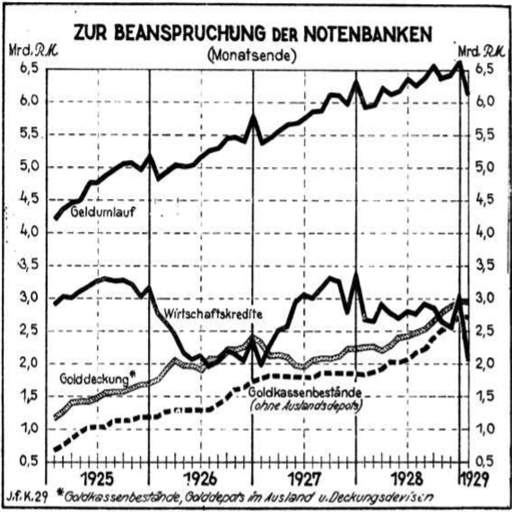
\includegraphics[width=\linewidth]{Methodik/img/lines_historical.png}
        \caption{\hbadness=10000 Historisches Liniendiagramm \phantom{Platzhalter}}
        \label{fig:lines_historical}
    \end{minipage}\hfill % Add space between figures
    \begin{minipage}{0.475\textwidth} % Second figure
        \centering
        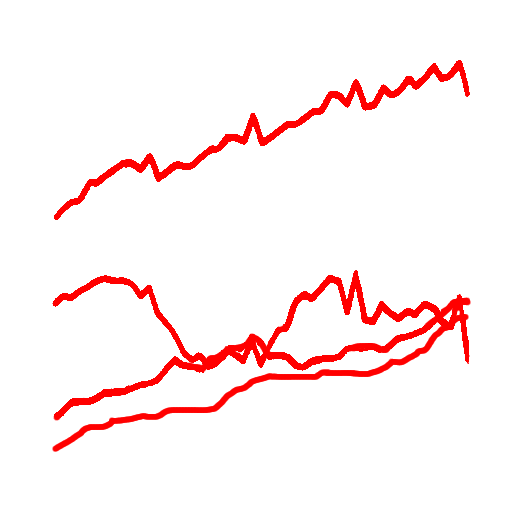
\includegraphics[width=\linewidth]{Methodik/img/lines_historical_mask.png}
        \caption{\hbadness=10000 Zugehörige manuell erstellte Binärmaske der Wertelinien}
        \label{fig:lines_historical_mask}
    \end{minipage}
\end{figure}

Die manuelle Erstellung der Wertelinienbinärmasken der historischen Liniendiagrammen fällt dagegen nicht ganz so leicht aus. Für die Anfertigung der Werteliniengrundwahrheiten wurde das Originalbild in einem Bildbearbeitungsprogramm \cite{photopea} geöffnet und pro Wertelinie eine eigene Bildschicht (layer) hinzugefügt. In jeder dieser einzelnen Schichten kann dann die jeweilige Wertelinine überzeichnet - abgepaust - werden. Der Grund jede Wertelinie in ihre eigene Maskenschicht zu übertragen ist der, dass am Ende einfach alle Schichten getrennt exportiert werden können. Für die semantische Segementation ist dies allerdings nicht nötig, da pro Klasse nur eine gemeinsame Binärmaske verwendet wird. Hier können jedoch dann ganz einfach alle exportierten Schichten in eine gemeinsame Maske vereinigt werden. In dem Fall der Instanzsegmentation dagegen wird eben nicht nur eine vereinigte Binärmaske pro Klase benötigt, sondern eine eigene Maske pro Objektinstanz - pro Wertelinie. Dementsprechend können hierfür die getrennten Maskenschichten verwendet werden. Werden hierfür wieder die Grundwahrheiten im Polygonannotationsformat erfordert, können diese, wie zuvor beschreiben, durch Konturerkennung von der Binärmask konvertiert werden.